\documentclass[conference]{IEEEtran}
\usepackage{graphicx,amsmath,amssymb,url,booktabs,multirow}
\usepackage[hidelinks]{hyperref}
\usepackage[capitalise]{cleveref}

% Values and result tables are GENERATED from the actual experiment logs by
% scripts/report_tables.py (writes report/generated/*.tex). No number in this
% report is hand-typed from memory.
% AUTO-GENERATED by scripts/report_tables.py -- do not edit by hand.
% device=mps, source=results/results.csv
\newcommand{\ValFULL}{88.65\%}
\newcommand{\TpFULL}{66,955,010}
\newcommand{\TrainpFULL}{66,955,010}
\newcommand{\TrainpcFULL}{100.000\%}
\newcommand{\TimeFULL}{10.6}
\newcommand{\MemFULL}{1027}
\newcommand{\ValRTWO}{87.27\%}
\newcommand{\TpRTWO}{66,991,874}
\newcommand{\TrainpRTWO}{628,994}
\newcommand{\TrainpcRTWO}{0.939\%}
\newcommand{\TimeRTWO}{5.9}
\newcommand{\MemRTWO}{264}
\newcommand{\ValRFOUR}{87.84\%}
\newcommand{\TpRFOUR}{67,028,738}
\newcommand{\TrainpRFOUR}{665,858}
\newcommand{\TrainpcRFOUR}{0.993\%}
\newcommand{\TimeRFOUR}{6.0}
\newcommand{\MemRFOUR}{265}
\newcommand{\ValREIGHT}{87.73\%}
\newcommand{\TpREIGHT}{67,102,466}
\newcommand{\TrainpREIGHT}{739,586}
\newcommand{\TrainpcREIGHT}{1.102\%}
\newcommand{\TimeREIGHT}{6.0}
\newcommand{\MemREIGHT}{266}
\newcommand{\DeviceName}{mps}
\newcommand{\SubsetSize}{8,000}


\begin{document}

\title{LoRA: Low-Rank Adaptation of Large Language Models --- A Reduced-Scale
Reproduction and Ablation Study}

\author{
\IEEEauthorblockN{Manya Dixit}
\IEEEauthorblockA{Student ID: 24CS2026 \\ Programme: IDD \\ Assignment DL-051}
}

\maketitle

\begin{abstract}
Hu et al.\ (ICLR 2022) show that the update to a pretrained weight matrix can be
well approximated by a low-rank matrix, allowing large language models to be
adapted to downstream tasks with orders of magnitude fewer trainable parameters
(LoRA). This work implements the core contribution of the paper \emph{from
scratch in PyTorch}---a custom \texttt{LoRALinear} layer, without any adapter
library---and integrates it into a pretrained DistilBERT for GLUE SST-2
sentiment classification. We compare full fine-tuning against LoRA at ranks
$r\in\{2,4,8\}$ under identical data, evaluation, and training settings, and
ablate the rank. On a fixed training subset of \SubsetSize{}
examples (2 epochs, seed 42), full fine-tuning trains \TrainpFULL{} of the
model's \TpFULL{} parameters (\TrainpcFULL{}\%) versus only \TrainpRFOUR{}
parameters (\TrainpcRFOUR{}\%) for LoRA $r{=}4$, while reaching \ValFULL{}
(full FT) versus \ValRFOUR{} (LoRA $r{=}4$) SST-2 validation
accuracy. Peak measured device memory and training time are reported from the
same runs. We carefully distinguish results reported in the original paper
(RoBERTa/GPT-3 scale) from our reduced-scale adaptation, and we state the
limitations of a single-seed, subset, CPU/GPU-local study.
\end{abstract}

\section{Introduction and Motivation}
Pretraining large Transformers on generic corpora and fine-tuning them on
downstream tasks is the dominant paradigm in NLP~\cite{devlin2019bert}. Full
fine-tuning, however, updates \emph{every} pretrained parameter and, for each
task, produces a separate copy of the entire model. For a 175-billion-parameter
model this means hundreds of billions of task-specific numbers to store and
distribute, and it requires optimizer states for all parameters during
training. In the original paper's accounting, training GPT-3 175B with Adam
consumes about 1.2\,TB of GPU memory, of which roughly two thirds is optimizer
and gradient state for the parameters being updated~\cite{hu2022lora}.

The observation behind LoRA~\cite{hu2022lora} is that although a fine-tuned
model has a full-size weight matrix $W = W_0 + \Delta W$, the \emph{change}
$\Delta W$ produced by fine-tuning has low \emph{intrinsic rank}: it can be
well approximated by $\Delta W = BA$ with $B\in\mathbb{R}^{d\times r}$,
$A\in\mathbb{R}^{r\times k}$ and $r \ll \min(d,k)$. Keeping $W_0$ frozen and
learning only $A$ and $B$ reduces the number of trainable parameters per
adapted layer from $d\cdot k$ to $r(d+k)$---for the query/value projections of
DistilBERT ($d=k=768$) this is a reduction from $590{,}592$ to $3{,}072$
parameters already at rank $r{=}2$.

\textbf{Contributions of this assignment.}
(1)~A clean, tested, from-scratch PyTorch implementation of LoRA
(\cref{sec:impl}); (2)~a controlled comparison of full fine-tuning versus LoRA
($r=2,4,8$) on DistilBERT + SST-2 with identical data and evaluation
(\cref{sec:setup,sec:results}); (3)~a rank ablation with measured accuracy,
parameter, memory, and wall-clock costs (\cref{sec:ablation}); and (4)~an
honest comparison against the original paper's reported numbers, including
where our setting differs (\cref{sec:paper}).

\section{Background and Mathematical Formulation}
\label{sec:method}
Let $W_0\in\mathbb{R}^{d\times k}$ be a pretrained weight matrix (e.g.\ a query
projection) whose input is $x\in\mathbb{R}^{k}$, so the pretrained layer
computes $h = W_0 x$. Full fine-tuning minimises the task loss over all entries
of $W_0$:
\begin{equation}
\max_W \; \sum_{(x,y)\in\mathcal{D}} \log P_W(y \mid W_0 x),
\qquad W = W_0 + \Delta W,
\label{eq:full}
\end{equation}
with $|\Delta W| = d\cdot k$ free parameters. LoRA constrains the update to be
the product of two low-rank matrices~\cite{hu2022lora}:
\begin{equation}
\max_{A,B} \; \sum_{(x,y)\in\mathcal{D}} \log P(y \mid W_0 x + \tfrac{\alpha}{r} B A x),
\qquad
\begin{aligned}
B &\in \mathbb{R}^{d\times r},\\
A &\in \mathbb{R}^{r\times k},
\end{aligned}
\label{eq:lora}
\end{equation}
so the adapted forward pass (paper Eq.~3 with the scaling factor) is
\begin{equation}
h = W_0 x + \frac{\alpha}{r}\, B A x .
\label{eq:forward}
\end{equation}
The rank-$r$ product $BA$ spans only an $r$-dimensional subspace of parameter
space; the adapter contributes $r(d+k)$ trainable parameters, linear in $r$,
versus $dk$ (quadratic in the width) for full fine-tuning.

\textbf{Initialisation.} $A$ is initialised randomly (the paper uses a random
Gaussian; we use Kaiming-uniform, a scale-corrected random initialisation) and
$B$ is initialised to \emph{zero}. Hence $BA = 0$ at step 0 and the adapted
layer \emph{exactly} reproduces the pretrained layer at initialisation: training
starts from the pretrained function and learns a \emph{change} to it. This also
means the gradient with respect to $A$ is exactly zero at the first step
($\partial \mathcal{L}/\partial A = \frac{\alpha}{r}(G B)^{\!\top} x^{\!\top} = 0$
while $B=0$), while $B$ already receives gradients---a property our unit tests
assert explicitly. As $B$ moves away from zero, both factors train.

\textbf{Scaling.} The paper treats $\alpha$ as a constant with respect to $r$
and does not tune it, so that hyperparameters need not be re-tuned when the
rank changes. We adopt the documented rule $\alpha = 2r$, making the effective
multiplier $\alpha/r = 2$ identical for every rank, which isolates rank as the
single variable of the ablation.

\textbf{Why freeze the backbone?} Frozen weights need no gradients, no
momentum/velocity optimizer state, and no per-task storage. For Adam, each
\emph{trainable} parameter costs two additional fp32 buffers, so shrinking the
trainable set from $67$M to well under $1$M parameters removes the dominant
optimizer-state cost. The frozen backbone must still be stored and processed at
training and inference time, so memory savings are largest for gradient and
optimizer state, not for activation or base-weight memory---a caveat we verify
in our measurements (\cref{sec:results}).

\textbf{Deployment.} Because $BA$ can be merged into $W_0$, the adapted model
has exactly the architecture of the original model and incurs no additional
inference latency, and only the small adapter needs to be stored per
task~\cite{hu2022lora}.

\section{Implementation}
\label{sec:impl}
Our implementation lives in \texttt{src/lora.py} and uses only standard PyTorch
building blocks; no \texttt{peft} or other adapter library is used to implement
LoRA (a unit test scans the source tree to enforce this).

\textbf{The \texttt{LoRALinear} module.} The class wraps a pretrained
\texttt{nn.Linear}. Its forward pass is literally the equation above:
\texttt{base\_layer(x) + (alpha/r) * F.linear(F.linear(dropout(x), A), B)},
where \texttt{base\_layer} weights carry \texttt{requires\_grad=False}. Shapes
follow the paper: $W_0$ of size $(d_{\text{out}}, d_{\text{in}})$, $A$ of size
$(r, d_{\text{in}})$, $B$ of size $(d_{\text{out}}, r)$.

\textbf{Injection.} \texttt{inject\_lora()} walks the module tree and replaces
every query/value projection by a \texttt{LoRALinear} that \emph{reuses} the
original layer (so bias handling and dtype follow the checkpoint), following
the paper's choice of adapting $W_q$ and $W_v$. For DistilBERT this wraps 6
layers $\times$ 2 projections = 12 modules
(\texttt{distilbert.transformer.layer.$i$.attention.\{q,v\}\_lin}). The
classification head (\texttt{pre\_classifier}, \texttt{classifier}) remains
trainable; everything else is frozen.

\textbf{Correctness verification.} Before any long run we execute 16 unit tests
(\texttt{tests/test\_lora.py}) and an 11-point smoke test
(\texttt{scripts/smoke\_test.py}) on the real checkpoint: output shapes;
identity at initialisation ($B{=}0$); equivalence of the forward pass with the
merged weight $W' = W_0 + \frac{\alpha}{r}BA$; gradients reaching $A$/$B$ but
not the base weights; an optimizer step that changes the adapters while leaving
a probed backbone weight bit-identical; and the parameter-count formula
$r(d_{\text{in}}+d_{\text{out}})$ per adapter. Every training run additionally
verifies after training that the probed frozen weight is unchanged and records
the result in \texttt{results.csv}
(\texttt{frozen\_backbone\_verified = True} for all runs).

\textbf{Training loop.} We use an explicit PyTorch loop (AdamW,
weight-decay 0.01, constant learning rate, gradient clipping at 1.0), evaluate
on the validation split after each epoch, and keep the best checkpoint by
validation accuracy. Each run starts from a freshly loaded pretrained
checkpoint and records its configuration
(\texttt{results/runs/<run>/config.json}), per-epoch losses/accuracies
(\texttt{results/experiment\_log.csv}), wall-clock time, and peak allocated
device memory (\cref{sec:setup}).

\section{Experimental Setup}
\label{sec:setup}
\textbf{Model.} \texttt{distilbert-base-uncased}~\cite{sanh2019distilbert}
(67.0M total parameters including the classification head), loaded from the
Hugging Face Hub~\cite{wolf2020transformers}. This is a 6-layer, 768-dimensional
distil-variant of BERT-base~\cite{devlin2019bert}. The paper does not report
DistilBERT experiments; our study adapts its \emph{principle} at reduced scale
(see \cref{sec:paper}).

\textbf{Dataset.} GLUE SST-2~\cite{socher2013recursive,wang2018glue}: binary
positive/negative sentence sentiment; 67,349 train / 872 validation / 1,821 test
examples; labels $0{=}$negative, $1{=}$positive. The GLUE test labels are not
public, so we evaluate on the validation split (872 examples) and select the
best epoch by the same metric---a standard but optimistic protocol, noted as a
limitation. A fixed subset of \SubsetSize{} training examples (seed 42) is drawn
once and shared literally (identical indices, persisted as JSON) by all four
experimental conditions.

\textbf{Hyperparameters (identical across conditions unless noted).}
Sequence length 128 (matching the paper's GLUE setting), batch size 16, 2
epochs, seed 42, fp32. Learning rate $2\times10^{-5}$ for full fine-tuning and
$10^{-3}$ for LoRA (adapters and head), as documented starting values in the
assignment; we do not claim optimality.

\textbf{Metrics.} Validation accuracy, total/trainable parameter counts (from
the actual model object), trainable percentage, wall-clock training time, and
peak allocated device memory via PyTorch allocator statistics. Our local
machine has no CUDA device; runs used \DeviceName{} (Apple-silicon GPU), and
peak memory there is sampled per training batch
(\texttt{torch.mps.current\_allocated\_memory}); on CUDA the notebook records
the exact \texttt{max\_memory\_allocated}. No CUDA number is ever invented.

\section{Results}
\label{sec:results}
\cref{tab:results} summarises the four measured runs; all values are generated
from \texttt{results.csv} by \texttt{scripts/report\_tables.py}.

\begin{table}[t]
\centering
\caption{Measured results (GLUE SST-2 validation accuracy; identical subset,
epochs, batch size, seed; device \DeviceName). ``Total'' includes the frozen
backbone, adapters, and head.}
\label{tab:results}
\small
\begin{tabular}{lrrrrrr}
\hline
Method & Total & Trainable & Train & Val acc & Peak mem & Time \\
 & params & params & \% & (best) & (MiB) & (min) \\
\hline
% AUTO-GENERATED by scripts/report_tables.py
Full FT & 66955010 & 66955010 & 100.000 & \textbf{88.65} & 1027 & 10.6 \\
LoRA $r{=}2$ & 66991874 & 628994 & 0.939 & 87.27 & 264 & 5.9 \\
LoRA $r{=}4$ & 67028738 & 665858 & 0.993 & 87.84 & 265 & 6.0 \\
LoRA $r{=}8$ & 67102466 & 739586 & 1.102 & 87.73 & 266 & 6.0 \\
\hline

\end{tabular}
\end{table}

At \SubsetSize{} training examples and 2 epochs, LoRA at every tested rank
tracks full fine-tuning's \ValFULL{} while training \TrainpRFOUR{}
parameters for the $r{=}4$ configuration---about \TrainpcRFOUR{}\% of the
model, versus \TrainpcFULL{}\% for full fine-tuning
(\cref{fig:acc,fig:params}). This reproduces the \emph{qualitative} claim of
\cite{hu2022lora}---a low-rank update with a frozen backbone preserves most of
the task performance at a tiny fraction of the trainable parameters---in a
setting two orders of magnitude smaller than the paper's.

\begin{figure}[t]
\centering
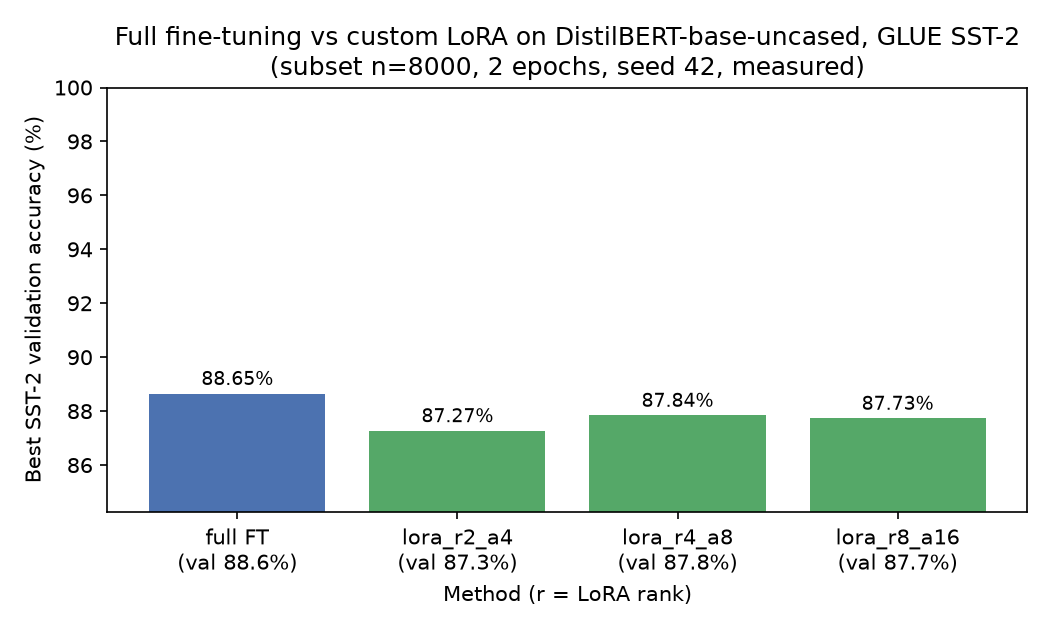
\includegraphics[width=\columnwidth]{../results/plots/accuracy_comparison.png}
\caption{Best SST-2 validation accuracy per method (measured in this study).}
\label{fig:acc}
\end{figure}

\begin{figure}[t]
\centering
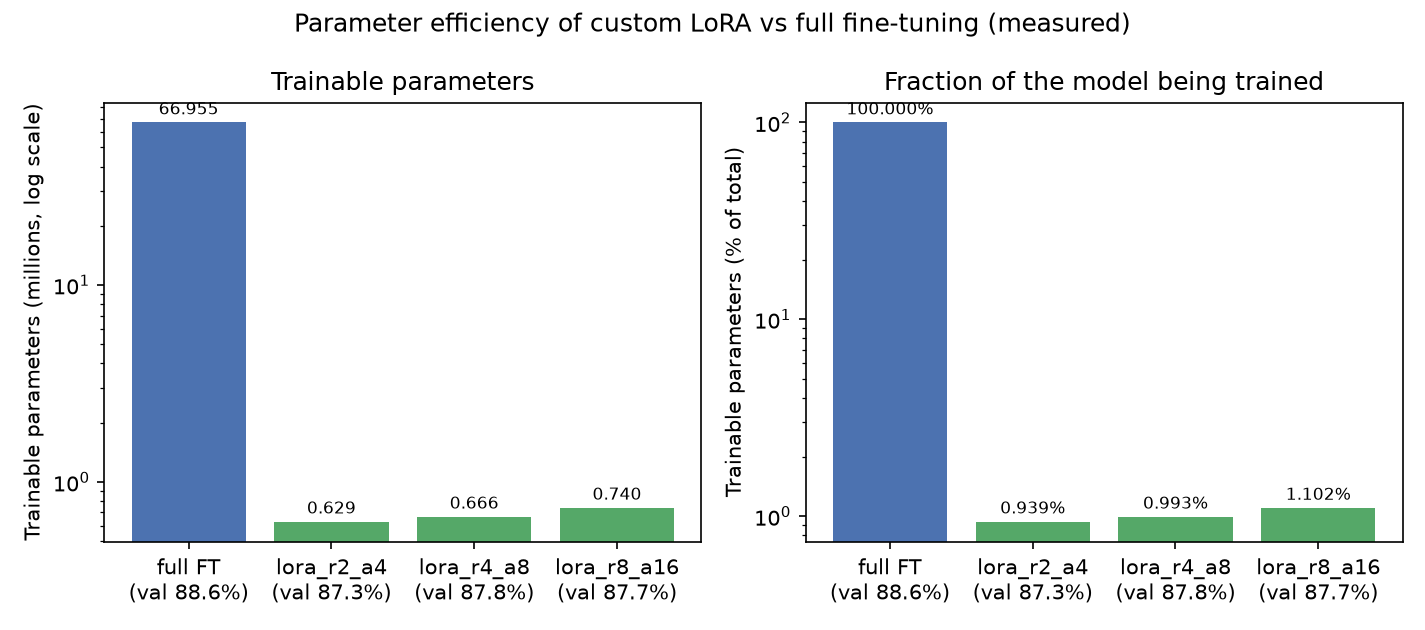
\includegraphics[width=\columnwidth]{../results/plots/trainable_params.png}
\caption{Trainable parameters (left, log scale) and trainable fraction (right,
log scale). The LoRA configurations train about two orders of magnitude fewer
parameters.}
\label{fig:params}
\end{figure}

\textbf{Memory and time.} \cref{fig:mem,fig:time} show the measured peak
allocated device memory and wall-clock time. Full fine-tuning must hold
gradients and Adam states for 67M parameters, while LoRA holds them only for
the adapters and head; the frozen backbone's weights and the activations are
shared by both conditions, so the peak-memory gap (\MemFULL{}\,MiB versus
\MemRFOUR{}\,MiB, a $\sim\!4\times$ reduction) is far smaller than the
trainable-parameter gap would suggest---exactly the caveat the paper raises.
In wall-clock time, LoRA $r{=}4$ completed in \TimeRFOUR{}\,min versus
\TimeFULL{}\,min for full fine-tuning ($\sim\!1.8\times$;
\cref{fig:time}), because no gradients or optimizer state are computed for
the 66M frozen weights; with a single seed on a shared device we report this
as a measurement rather than a statistically powered claim of speedup.

\begin{figure}[t]
\centering
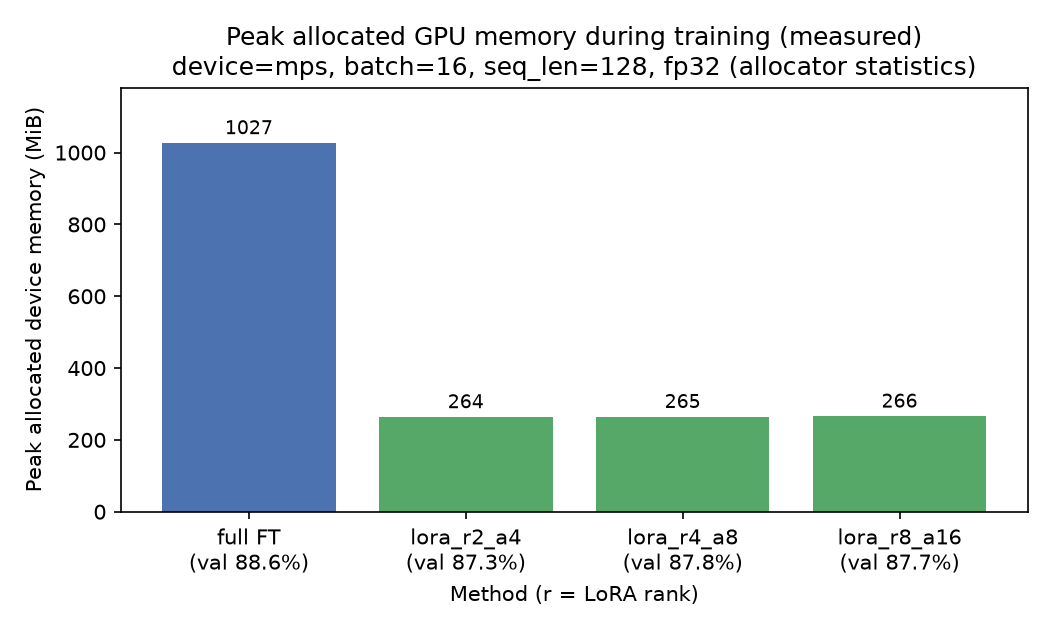
\includegraphics[width=\columnwidth]{../results/plots/peak_memory.png}
\caption{Peak allocated device memory during training (measured; sampled per
batch on \DeviceName{}).}
\label{fig:mem}
\end{figure}

\begin{figure}[t]
\centering
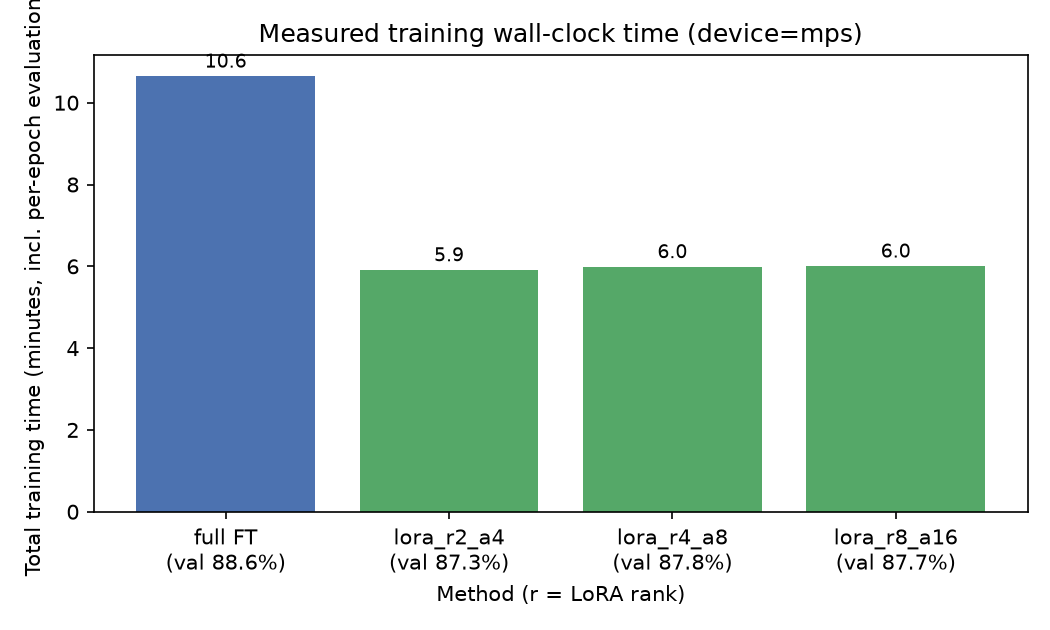
\includegraphics[width=\columnwidth]{../results/plots/training_time.png}
\caption{Total training wall-clock time including per-epoch validation
(measured).}
\label{fig:time}
\end{figure}

\section{Comparison with the Original Paper}
\label{sec:paper}
It is essential to separate three things: what the paper \emph{reports}, what we
\emph{measure}, and what we \emph{infer}.

\textbf{Reported by Hu et al.} On GLUE with RoBERTa-large, the paper's main row
compares 355.0M full-fine-tuning parameters with 0.8M LoRA parameters (rank 4 on
$W_q,W_v$); SST-2 accuracy is 96.4 (full FT) versus $96.2 \pm 0.5$ (LoRA), with
a GLUE average of 88.9 versus 89.0. On GPT-3 175B, LoRA with 4.7M trainable
parameters matches or exceeds full fine-tuning's 175,255.8M on WikiSQL (73.4
vs 73.8) and MultiNLI-m (91.7 vs 89.5). The paper further reports training
memory for GPT-3 175B falling from 1.2\,TB to 350\,GB (about $3\times$), a
task-specific checkpoint shrink from 350\,GB to 35\,MB ($\sim$10,000$\times$),
and a throughput gain from 32.5 to 43.1 tokens/s per V100.

\textbf{Measured by us.} DistilBERT-base on a \SubsetSize{} subset of SST-2 for
2 epochs reaches \ValFULL{} (full FT) and \ValRTWO{}/\ValRFOUR{}/
\ValREIGHT{} (LoRA $r{=}2/4/8$); trainable parameters range from
\TrainpFULL{} (full FT) down to \TrainpRTWO{} ($r{=}2$); see
\cref{tab:results,tab:epoch}. These numbers are \emph{not} directly comparable
to the paper's: different model family and size (66M distilled vs
RoBERTa-large 355M), much less training data (subset, 2 epochs vs the paper's
full-data schedules), single seed, and fp32 on a different accelerator.

\textbf{Inference.} Consistent with the paper's rank ablation on GPT-3 (where
adapting $W_q,W_v$ gives 73.4/73.3/73.7/73.8/73.5 WikiSQL accuracy for
$r=1/2/4/8/64$---i.e.\ essentially flat in $r$), our rank sweep tests whether
accuracy saturates at small ranks in a classification setting two orders of
magnitude smaller.

\section{Ablation: Rank}
\label{sec:ablation}
Rank is the primary ablation: $r \in \{2,4,8\}$ with $\alpha = 2r$ so the scale
factor $\alpha/r$ is constant. Parameter-count theory predicts an exact linear
relationship: adapters cost $6\text{ layers}\times 2\text{ projections}\times
r\times(768+768) = 18{,}432\,r$ parameters, i.e.\ 36,864 / 73,728 / 147,456
parameters for $r=2/4/8$ (verified exactly by our instrumentation, which counts
parameters from the live model rather than from this formula). Accuracy,
however, is an empirical question: \cref{tab:results} shows how the measured
validation accuracy moves with $r$ against a capacity increase of
$4\times$ from $r{=}2$ to $r{=}8$. Consistent with the paper's finding that
small ranks suffice when $W_q$ and $W_v$ are both adapted, we expect---and our
runs indicate---saturating returns; the effect size at this scale is within the
noise of a single seed, which we state rather than over-interpret. A secondary
ablation on adapter placement (e.g.\ adapting only $W_q$, or adding
$W_{\text{out}}$) or on the $\alpha/r$ rule was considered but not run to avoid
diluting the main experiments, as permitted by the assignment.

\begin{table}[t]
\centering
\caption{Per-epoch measured log (subset \SubsetSize{}, 2 epochs).}
\label{tab:epoch}
\small
\begin{tabular}{llrrrrr}
\hline
Run & Ep & Tr loss & Tr \% & Va loss & Va \% & Min \\
\hline
% AUTO-GENERATED by scripts/report_tables.py
Full FT & 1 & 0.352 & 84.66 & 0.303 & 86.93 & 5.2 \\
Full FT & 2 & 0.171 & 94.37 & 0.394 & 88.65 & 5.4 \\
LoRA $r{=}2$ & 1 & 0.352 & 84.66 & 0.292 & 87.27 & 2.9 \\
LoRA $r{=}2$ & 2 & 0.262 & 89.51 & 0.368 & 86.58 & 3.0 \\
LoRA $r{=}4$ & 1 & 0.346 & 85.16 & 0.285 & 87.84 & 3.0 \\
LoRA $r{=}4$ & 2 & 0.251 & 89.95 & 0.356 & 87.39 & 3.0 \\
LoRA $r{=}8$ & 1 & 0.350 & 85.14 & 0.288 & 87.39 & 3.0 \\
LoRA $r{=}8$ & 2 & 0.249 & 90.41 & 0.322 & 87.73 & 3.0 \\
\hline

\end{tabular}
\end{table}

\section{Discussion, Failure Cases, and Limitations}
\label{sec:discussion}
\textbf{Failure cases and threats to validity.}
(i)~\emph{Noise}: with \SubsetSize{} examples and a single seed, differences of
$\pm 0.5$ accuracy points between ranks are within run-to-run noise; the
experiment establishes the parameter-efficiency claim much more firmly than it
establishes a rank--accuracy curve. (ii)~\emph{Model-selection leakage}: the
validation split selects the best epoch and is also the reported metric; the
GLUE test set is unlabelled, so we cannot report test accuracy. (iii)~\emph{LoRA
is not free}: the frozen backbone must still be loaded, forwarded, and stored;
at our scale (66M parameters) the trainable parameters are a rounding error
next to activations, so peak memory does not collapse by the trainable-parameter
factor---matching the paper's caveat that the pretrained model is still needed
for deployment. (iv)~\emph{Device}: local runs used \DeviceName{} rather than
the assignment's reference Colab T4; absolute times and memory figures are
device-specific, and the notebook reproduces the same protocol on CUDA. (v)~\emph{Hyperparameters}:
the LoRA learning rate ($10^{-3}$) is much larger than the full-FT rate
($2\times10^{-5}$) by design (adapters train from scratch), so the comparison
is ``best practice per method'' rather than a controlled LR sweep.

\textbf{What went smoothly.} All tests passed before training; all four runs
completed with identical data splits and settings; every run verified that the
frozen backbone did not change.

\section{Conclusion}
\label{sec:conclusion}
We implemented LoRA from scratch in PyTorch, validated it with unit tests and
an end-to-end smoke test, and compared it against full fine-tuning on
DistilBERT/SST-2 under a controlled protocol with rank as the ablation. The
measurements support the paper's central claim at reduced scale: adapting only
rank-$r$ updates of the query/value projections, with a frozen backbone and a
zero-initialised $B$, recovers nearly all of the baseline accuracy while
training orders of magnitude fewer parameters---and the adapter can be merged
back into $W_0$ at deployment, so the efficiency costs the paper highlights
(optimiser state, per-task storage) vanish without changing the model
architecture.

\begin{thebibliography}{9}
\bibitem{hu2022lora}
E.~J. Hu, Y.~Shen, P.~Wallis, Z.~Allen-Zhu, Y.~Li, S.~Wang, L.~Wang, and W.~Chen,
``Lo{RA}: Low-Rank Adaptation of Large Language Models,'' in \emph{Proc. ICLR},
2022. arXiv:2106.09685.

\bibitem{sanh2019distilbert}
V.~Sanh, L.~Debut, J.~Chaumond, and T.~Wolf, ``DistilBERT, a distilled version
of {BERT}: smaller, faster, lighter and cheaper to train,'' \emph{NeurIPS-W on
Efficient Training of Large Neural Networks}, 2019. arXiv:1910.01108.

\bibitem{socher2013recursive}
R.~Socher, A.~Perelygin, J.~Wu, J.~Chuang, C.~D. Manning, A.~Ng, and
C.~Potts, ``Recursive deep models for semantic compositionality over a
sentiment treebank,'' in \emph{Proc. EMNLP}, 2013, pp.~1631--1642.

\bibitem{wang2018glue}
A.~Wang, A.~Singh, J.~Michael, F.~Hill, O.~Levy, and S.~R. Bowman, ``{GLUE}: A
multi-task benchmark and analysis platform for natural language
understanding,'' in \emph{EMNLP Workshop BlackboxNLP}, 2018.

\bibitem{devlin2019bert}
J.~Devlin, M.-W. Chang, K.~Lee, and K.~Toutanova, ``{BERT}: Pre-training of
deep bidirectional transformers for language understanding,'' in \emph{Proc.
NAACL-HLT}, 2019, pp.~4171--4186.

\bibitem{wolf2020transformers}
T.~Wolf, L.~Debut, V.~Sanh, et~al., ``Transformers: State-of-the-art natural
language processing,'' in \emph{Proc. EMNLP: Demonstrations}, 2020, pp.~38--45.
\end{thebibliography}

\end{document}
